\chapter{Fundamentos Geofísicos}
\label{cha:fundamentos}

\section{Campo potencial gravitatorio}

Según la Ley de Gravitación Universal de Newton, una masa puntual $m_p$ situada
en la posición $\mathbf{p}$ se ve sometida una fuerza gravitatoria $\mathbf{F}$
debido a la presencia de otra masa $m$ situada en la posición $\mathbf{q}$.
Esta fuerza puede expresarse como:

\begin{equation}
    \mathbf{F} =
        - G
        \frac{m_p m}{\left\lVert \mathbf{p} - \mathbf{q}\right\rVert^3}
        (\mathbf{p} - \mathbf{q}),
\end{equation}

\noindent donde $G = 6.67430 \times 10^{-11} \text{m}^3 \text{kg}^{-1}
\text{s}^{-2}$ es la constante de gravitación universal
(Fig.~\ref{fig:potencial-gravitatorio}a) y $\left\lVert \cdot \right\rVert$
representa la norma L$_2$.
Aplicando la segunda Ley de Newton, se deduce que la masa $m_p$ experimenta una
aceleración gravitatoria $\mathbf{g}$:

\begin{equation}
    \mathbf{g} =
        - \frac{G m}{\left\lVert \mathbf{p} - \mathbf{q} \right\rVert^3}
        (\mathbf{p} - \mathbf{q}).
    \label{eq:aceleracion-newton}
\end{equation}

Si consideramos que la partícula $m_p$ es una \emph{partícula de prueba},
podemos reescribir la ecuación \ref{eq:aceleracion-newton}, pero ahora
resignificándola como la aceleración gravitatoria que sentiría cualquier
partícula localizada en un punto $\mathbf{p}$ debido a la presencia de la
partícula $m$:

\begin{equation}
    \mathbf{g}(\mathbf{p}) =
        - \frac{G m}{\left\lVert \mathbf{p} - \mathbf{q} \right\rVert^3}
        (\mathbf{p} - \mathbf{q}).
\end{equation}

Se puede demostrar que la atracción gravitatoria $\mathbf{g}$ define un campo
irrotacional, es decir:

\begin{equation}
    \nabla \times \mathbf{g} = 0.
\end{equation}

\noindent Por ende es posible definir un potencial escalar $V$ al que
denominaremos \emph{potencial gravitatorio}:

\begin{equation}
    \mathbf{g}(\mathbf{p}) = + \nabla V(\mathbf{p}),
    \label{eq:potencial-gravitatorio-definicion}
\end{equation}

\noindent donde

\begin{equation}
    V(\mathbf{p}) =
      G \frac{m}{\left\lVert \mathbf{p} - \mathbf{q} \right\rVert}.
    \label{eq:potencial-gravitatorio-particula}
\end{equation}

\noindent Vale la pena notar que en la ecuación
\ref{eq:potencial-gravitatorio-definicion} se ha aplicado la convención de
signo positivo para definir el potencial $V$, mayormente utilizada en la
literatura sobre Geofísica y Geodesia
\citep{heiskanen1967,blakely1995,hinze2009}.

\begin{figure}
    \centering
    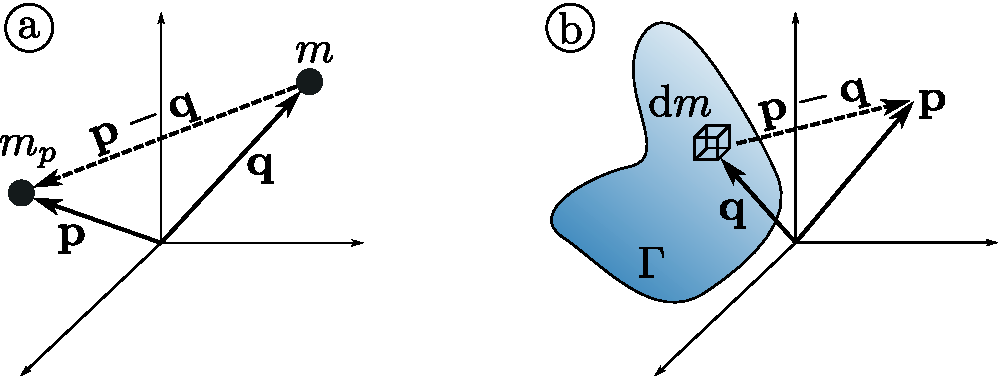
\includegraphics[width=\linewidth]{figs/gravity-potentials.pdf}
    \caption{
        (a)~Masas puntuales $m_p$ y $m$ localizadas en $\mathbf{p}$
        y $\mathbf{q}$, respectivamente.
        (b)~Distribución de masa $\Omega$, diferencial de masa $\diff m$
        ubicado en el punto $\mathbf{q}$.
    }
    \label{fig:potencial-gravitatorio}
\end{figure}


\subsection{Potencial gravitatorio por una distribución de masa}

Partiendo de que un diferencial de masa $\diff m$ ubicado en $\mathbf{q}$
genera un potencial gravitatorio $\diff V$ en cualquier punto $\mathbf{p}$
(Fig.~\ref{fig:potencial-gravitatorio}b):

\begin{equation}
    \diff V(\mathbf{p}) = \frac{G}{\left\lVert \mathbf{p} - \mathbf{q}
        \right\rVert} \diff m,
\end{equation}

\noindent el potencial gravitatorio generado por una distribución de masa
$\Omega$ puede calcularse integrando los diferenciales de masa que lo componen:

\begin{equation}
    V(\mathbf{p}) =
        G \int\limits_\Omega \frac{\diff m}{\left\lVert \mathbf{p} - \mathbf{q}
            \right\rVert} .
\end{equation}

Si reescribimos los diferenciales de masa como

\begin{equation}
    \diff m = \rho(\mathbf{q}) \diff v,
\end{equation}

\noindent donde $\rho(\mathbf{q})$ es la densidad de masa de la distribución
$\Omega$ en el punto $\mathbf{q}$ y $\diff v$ es el diferencial de volumen,
el potencial se puede expresar como:

\begin{equation}
    V(\mathbf{p}) =
        G \int\limits_\Omega
        \frac{\rho(\mathbf{q})}{\left\lVert \mathbf{p} - \mathbf{q}
            \right\rVert} \diff v.
    \label{eq:potencial-gravitatorio-integral}
\end{equation}


\subsection{Gradiente del potencial gravitatorio}

Según la definición del potencial gravitatorio expuesta en la
ecuación~\ref{eq:potencial-gravitatorio-definicion}, es posible calcular la
aceleración de la gravedad producida por una distribución de masa arbitraria
en cualquier punto $\mathbf{p}$ como el gradiente del potencial
$V(\mathbf{p})$.
Si definimos un sistema de ejes Cartesianos en el cual el punto $\mathbf{p}
= (x, y, z)$, las componentes de la aceleración en cada una de las direcciones
del sistema quedan expresadas
como:

\begin{equation}
    g_i(\mathbf{p}) = \frac{\partial V(\mathbf{p})}{\partial i}, \,\,
        \forall i \in \{x, y, z\}.
    \label{eq:componentes-aceleracion-gravitatoria}
\end{equation}

El vector
$\mathbf{g}(\mathbf{p}) = (g_x(\mathbf{p}), g_y(\mathbf{p}), g_z(\mathbf{p}))$
representa la aceleración gravitatoria en el punto
$\mathbf{p}$ generada por la distribución de masa $\Omega$, aunque es común
referirse al mismo como el \emph{gradiente gravitatorio}.
Reemplazando la ecuación~\ref{eq:potencial-gravitatorio-integral}
en~\ref{eq:componentes-aceleracion-gravitatoria}, las componentes del gradiente
gravitatorio pueden expresarse como:

\begin{align}
    g_x(\mathbf{p}) &=
        - G \int\limits_\Omega \rho(\mathbf{q})
        \frac{(x - x')}{\left\lVert \mathbf{p} - \mathbf{q} \right\rVert^3}
        \diff v,
    \label{eq:gx-integral}
    \\
    g_y(\mathbf{p}) &=
        - G \int\limits_\Omega \rho(\mathbf{q})
        \frac{(y - y')}{\left\lVert \mathbf{p} - \mathbf{q} \right\rVert^3}
        \diff v,
    \label{eq:gy-integral}
    \\
    g_z(\mathbf{p}) &=
        - G \int\limits_\Omega \rho(\mathbf{q})
        \frac{(z - z')}{\left\lVert \mathbf{p} - \mathbf{q} \right\rVert^3}
        \diff v,
    \label{eq:gz-integral}
\end{align}

\noindent donde $\mathbf{q} = (x', y', z')$.

Las segundas derivadas del potencial gravitatorio definen el \emph{tensor del
gradiente gravitatorio}, y sus componentes pueden expresarse como:

\begin{equation}
    g_{ij}(\mathbf{p}) =
        \frac{\partial^2 V(\mathbf{p})}{\partial i \partial j}, \,\,
        \forall i \in \{x, y, z\}, \,\,
        \forall j \in \{x, y, z\}.
\end{equation}

Reemplazando la ecuación \ref{eq:potencial-gravitatorio-integral}, podemos
expresar las componentes diagonales del tensor de la siguiente manera
\citep{grombein2013}:

\begin{align}
    g_{xx}(\mathbf{p}) &=
        G \int\limits_\Omega \rho(\mathbf{q})
        \left[
        \frac{3(x - x')^2}{\left\lVert \mathbf{p} - \mathbf{q} \right\rVert^5}
        - \frac{1}{\left\lVert \mathbf{p} - \mathbf{q} \right\rVert^3}
        \right]
        \diff v,
    \label{eq:gxx-integral}
    \\
    g_{yy}(\mathbf{p}) &=
        G \int\limits_\Omega \rho(\mathbf{q})
        \left[
        \frac{3(y - y')^2}{\left\lVert \mathbf{p} - \mathbf{q} \right\rVert^5}
        - \frac{1}{\left\lVert \mathbf{p} - \mathbf{q} \right\rVert^3}
        \right]
        \diff v,
    \label{eq:gyy-integral}
    \\
    g_{zz}(\mathbf{p}) &=
        G \int\limits_\Omega \rho(\mathbf{q})
        \left[
        \frac{3(z - z')^2}{\left\lVert \mathbf{p} - \mathbf{q} \right\rVert^5}
        - \frac{1}{\left\lVert \mathbf{p} - \mathbf{q} \right\rVert^3}
        \right]
        \diff v,
    \label{eq:gzz-integral}
\end{align}

\noindent mientras que las componentes no diagonales pueden expresarse como:

\begin{align}
    g_{xy}(\mathbf{p}) =
    g_{yx}(\mathbf{p}) &=
        G \int\limits_\Omega \rho(\mathbf{q})
        \frac{
            3(x - x')(y - y')
        }{
            \left\lVert \mathbf{p} - \mathbf{q} \right\rVert^5
        }
        \diff v,
    \label{eq:gxy-integral}
    \\
    g_{xz}(\mathbf{p}) =
    g_{zx}(\mathbf{p}) &=
        G \int\limits_\Omega \rho(\mathbf{q})
        \frac{
            3(x - x')(z - z')
        }{
            \left\lVert \mathbf{p} - \mathbf{q} \right\rVert^5
        }
        \diff v,
    \label{eq:gxz-integral}
    \\
    g_{yz}(\mathbf{p}) =
    g_{zy}(\mathbf{p}) &=
        G \int\limits_\Omega \rho(\mathbf{q})
        \frac{
            3(y - y')(z - z')
        }{
            \left\lVert \mathbf{p} - \mathbf{q} \right\rVert^5
        }
        \diff v.
    \label{eq:gyz-integral}
\end{align}

A partir de las ecuaciones~\ref{eq:gxx-integral}--\ref{eq:gzz-integral} podemos
calcular el Laplaciano del potencial gravitatorio:

\begin{equation}
    \nabla^2 V(\mathbf{p}) =
        \frac{\partial^2 V}{\partial x^2}
        + \frac{\partial^2 V}{\partial y^2}
        + \frac{\partial^2 V}{\partial z^2},
\end{equation}

\noindent Dado que las tres expresiones se cancelan mutuamente
\citep{blakely1995}, podemos concluir que cualquier potencial gravitatorio es
un \emph{campo harmónico}

\begin{equation}
    \nabla^2 V(\mathbf{p}) = 0
    \label{eq:potencial-laplace}
\end{equation}

\noindent para cualquier punto de observación $\mathbf{p}$ fuera de la
distribución de masa $\Omega$.

Vale notar que la ecuación de Laplace \ref{eq:potencial-laplace} es válida
solo para regiones libres de masas, y representa un caso particular de la
ecuación de Poisson \citep{blakely1995}:

\begin{equation}
    \nabla^2 V(\mathbf{p}) = -4\pi G \, \rho(\mathbf{p}),
    \label{eq:potencial-poisson}
\end{equation}

\noindent válida para cualquier punto de observación $\mathbf{p}$.

% =============================================================================

\section{Modelado directo}

El cálculo de los efectos gravitatorios de un determinado cuerpo sobre uno
o más puntos de observación se suele denominar modelado directo (\emph{forward
modelling} en inglés).
Aunque las expresiones del potencial gravitatorio
(ec.~\ref{eq:potencial-gravitatorio-integral}),
las componentes de su gradiente
(ecs.~\ref{eq:gx-integral}--\ref{eq:gz-integral})
y de su tensor (ecs.~\ref{eq:gxx-integral}--\ref{eq:gzz-integral})
aparentan ser sencillas, el cómputo de estas magnitudes para una geometría dada
no resulta un problema trivial.
Solo existen soluciones analíticas a dichas expresiones para determinadas
geometrías sencillas o que guardan algún tipo de simetría.

En el desarrollo de esta Tesis nos resultan de principal interés trabajar con
tres tipos de geometrías: masas puntuales, prismas rectangulares y prismas
esféricos o \emph{tesseroides}.

\subsection{Masas puntuales}

La distribución de densidades de una masa puntual puede expresarse
sencillamente mediante una Delta de Dirac \citep{vladimirov1979}:

\begin{equation}
    \rho(\mathbf{q}) = m \, \delta(\mathbf{q} - \mathbf{q'}),
\end{equation}

\noindent donde $\mathbf{q}$ y $m$ son la posición y la masa de la partícula,
respectivamente.
Reemplazando esta expresión en la
ecuación~\ref{eq:potencial-gravitatorio-integral}, obtenemos el potencial
gravitatorio generado por una partícula:

\begin{equation}
    V(\mathbf{p}) =
        G \int\limits_\Omega
        m \frac{\delta(\mathbf{q} - \mathbf{q'})}{\left\lVert \mathbf{p}
            - \mathbf{q'} \right\rVert}
        \diff v =
        \frac{G m}{\left\lVert \mathbf{p} - \mathbf{q} \right\rVert},
    \label{eq:potencial-masa-puntual}
\end{equation}

\noindent de acuerdo con la expresión del potencial de la
ecuación~\ref{eq:potencial-gravitatorio-particula}.

Realizando el mismo reemplazo en las ecuaciones correspondientes a las
componentes del gradiente (ecs.~\ref{eq:gx-integral}--\ref{eq:gz-integral})
arribamos a las siguientes expresiones:

\begin{align}
    g_x(\mathbf{p}) &=
        - G m
        \frac{x - x'}{\left\lVert \mathbf{p} - \mathbf{q} \right\rVert^3},
    \label{eq:gx-particula}
    \\
    g_y(\mathbf{p}) &=
        - G m
        \frac{y - y'}{\left\lVert \mathbf{p} - \mathbf{q} \right\rVert^3},
    \label{eq:gy-particula}
    \\
    g_z(\mathbf{p}) &=
        - G m
        \frac{z - z'}{\left\lVert \mathbf{p} - \mathbf{q} \right\rVert^3}.
    \label{eq:gz-particula}
\end{align}

A la hora de realizar el cómputo de los campos gravitatorios de masas
puntuales, las posiciones de las partículas como de los puntos de observación
pueden venir dados en diferentes sistemas de coordenadas.
En el caso de necesitar modelar cualquier conjunto de masas situadas bajo la
superficie terrestre, resulta natural utilizar coordenadas esféricas tanto para
las posiciones de las partículas como para los puntos de observación.
Sin embargo, es muy común trabajar sobre zonas de estudio con dimensiones
acotadas, bajo las cuales la aproximación de Tierra plana es suficiente. En
estos casos es posible trabajar en coordenadas Cartesianas.

\subsubsection{Coordenadas Cartesianas}

En el caso de que la posición de la partícula venga dada por el vector
$\mathbf{q} = (x', y', z')$ y el punto de observación por el vector
$\mathbf{p} = (x, y, z)$ definidos en el mismo sistema de ejes Cartesianos, el
módulo de
$\mathbf{p} - \mathbf{q}$ se calcula sencillamente bajo la norma L$_2$:

\begin{equation}
    \left\lVert  \mathbf{p} - \mathbf{q}  \right\rVert = \sqrt{
        (x - x')^2 + (y - y')^2 + (z - z')^2
    }.
\end{equation}

Dado que los numeradores en las
ecuaciones~\ref{eq:gx-particula}--\ref{eq:gz-particula} resultan triviales en
coordenadas Cartesianas, el cómputo del potencial y las componentes de su
gradiente se puede realizar de manera sencilla.

\subsubsection{Coordenadas esféricas}

Consideremos que las posiciones del punto de observación y de la partícula
vienen dados en un sistema de coordenadas esféricas. Para ello vamos a definir
un sistema de referencia \emph{geocéntrico} $\{X, Y, Z\}$ y a partir del mismo
un sistema de coordenadas esféricas $\{r, \lambda, \phi\}$, donde $r$ es la
posición \emph{radial}, $\lambda$ la posición \emph{longitudinal} y $\phi$ la
posición \emph{latitudinal} (Fig.~\ref{fig:spherical-coordinates}).
Cualquier punto dado por las coordenadas esféricas $(r, \lambda, \phi)$ se
puede expresar en coordenadas Cartesianas geocéntricas bajo las siguientes
relaciones:

\begin{equation}
    \begin{cases}
        X = r \cos\lambda \cos{\phi} \\
        Y = r \sin\lambda \cos{\phi} \\
        Z = r \sin{\phi},
    \end{cases}
\end{equation}

\noindent donde $r \in [0, \infty)$, $\lambda \in (-\pi, \pi]$ y
$\phi \in [-\pi/2, \pi/2]$.

\begin{figure}[t]
    \centering
    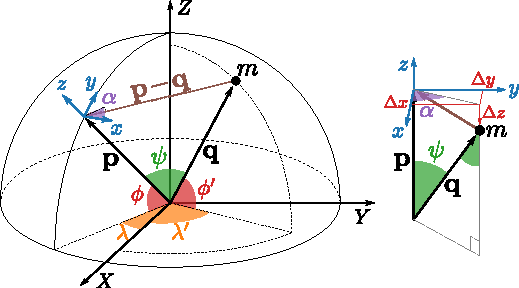
\includegraphics[width=\linewidth]{figs/spherical-coordinates.pdf}
    \caption{
        Masa puntual $m$ ubicada en la posición $\mathbf{q}$ y punto de
        observación situado en $\mathbf{p}$.
        Se define un sistema de referencia Cartesiano \emph{geocéntrico} $X, Y,
        Z$ bajo el cual se considera un sistema de coordenadas esféricas dadas
        por la distancia radial ($r$), ángulo longitudinal ($\lambda$) y ángulo
        latitudinal ($\phi$).
        En el punto $\mathbf{p}$ se define un sistema \emph{local} de
        coordenadas Cartesiano: el eje $x$ apunta hacia el Este,
        el eje $y$ hacia el Norte geométrico y el eje $z$ en la dirección
        radial.
        Se define a $\psi$ como el ángulo descripto por los vectores
        $\mathbf{p}$ y $\mathbf{q}$, y $\alpha$ al ángulo azimutal de
        $\mathbf{q} - \mathbf{p}$ sobre el sistema \emph{local}.
    }
    \label{fig:spherical-coordinates}
\end{figure}

El potencial gravitatorio que genera la partícula $m$ sobre el punto de
observación $\mathbf{p}$ puede calcularse mediante la
ecuación~\ref{eq:potencial-gravitatorio-particula}.
Considerando que los vectores $\mathbf{p}$ y $\mathbf{q}$ vienen definidos por
las coordenadas esféricas $(r, \lambda, \phi)$ y $(r', \lambda', \phi')$,
respectivamente, la distancia Euclidiana entre ellos puede expresarse como
\citep{grombein2013}:

\begin{equation}
    \left\lVert \mathbf{p} - \mathbf{q} \right\rVert = \sqrt{
        r^2 + r'^2 - 2rr'\cos\psi
    },
    \label{eq:distance-spherical}
\end{equation}

\noindent donde $\psi$ es el ángulo que describen los vectores $\mathbf{p}$
y $\mathbf{q}$:

\begin{equation}
    \cos \psi =
        \sin \phi \sin \phi' + \cos \phi \cos \phi' \cos(\lambda - \lambda').
    \label{eq:cosphi}
\end{equation}

La determinación de las componentes del gradiente del potencial gravitatorio
hace necesario que definamos las direcciones ortogonales $x$, $y$ y $z$ a lo
largo de las cuales se calculan las derivadas parciales de $V(\mathbf{p})$.
La elección más natural es obtener el gradiente con respecto a un sistema de
coordenadas \emph{local} $\{x, y, z\}$ \citep{grombein2013,uieda2016} donde $x$
se orienta en la dirección longitudinal (Este), $y$ en la dirección latitudinal
(Norte) y $z$ en la dirección radial.

Los numeradores de las ecuaciones~\ref{eq:gx-particula}--\ref{eq:gz-particula}
pueden expresarse en términos de las coordenadas esféricas como:

\begin{align}
    \Delta x &= - (x - x') = r' \sin\psi \cos\alpha
    \label{eq:delta-x-raw}
    \\
    \Delta y &= - (y - y') = r' \sin\psi \sin\alpha
    \label{eq:delta-y-raw}
    \\
    \Delta z &= - (z - z') = r'\cos\psi - r,
    \label{eq:delta-z-raw}
\end{align}

\noindent donde $\alpha$ es el ángulo azimutal del vector
$\mathbf{q} - \mathbf{p}$ sobre el sistema de coordenadas \emph{locales}.
Haciendo uso de las siguientes relaciones de trigonometría esférica
\citep[][p.~113]{heiskanen1967}:

\begin{align}
    \sin\psi \cos\alpha &=
        \cos\phi \sin\phi' - \sin\phi \cos\phi' \cos(\lambda - \lambda') \\
    \sin\psi \sin\alpha &=
        \cos\phi' \sin(\lambda - \lambda'),
\end{align}

\noindent podemos expresar las ecuaciones~\ref{eq:delta-x-raw},
\ref{eq:delta-y-raw} y \ref{eq:delta-z-raw} como \citep{grombein2013}:

\begin{align}
    \Delta x &= r' \sin\psi \left[
        \cos\phi \sin\phi' - \sin\phi \cos\phi' \cos(\lambda - \lambda')
        \right]
    \label{eq:delta-x}
    \\
    \Delta y &= r' \cos\phi' \sin(\lambda - \lambda')
    \label{eq:delta-y}
    \\
    \Delta z &= r'\cos\psi - r.
    \label{eq:delta-z}
\end{align}

Las componentes del gradiente del potencial gravitatorio generado por una masa
puntual en coordenadas esféricas quedan determinadas de la siguiente manera:

\begin{align}
    g_x(\mathbf{p}) &=
        G m
        \frac{\Delta x}{\left\lVert \mathbf{p} - \mathbf{q} \right\rVert^3},
    \label{eq:gx-particula-spherical}
    \\
    g_y(\mathbf{p}) &=
        G m
        \frac{\Delta y}{\left\lVert \mathbf{p} - \mathbf{q} \right\rVert^3},
    \label{eq:gy-particula-spherical}
    \\
    g_z(\mathbf{p}) &=
        G m
        \frac{\Delta z}{\left\lVert \mathbf{p} - \mathbf{q} \right\rVert^3},
    \label{eq:gz-particula-spherical}
\end{align}

\noindent haciendo uso de las ecuaciones~\ref{eq:distance-spherical},
\ref{eq:cosphi}, \ref{eq:delta-x}, \ref{eq:delta-y} y \ref{eq:delta-z}.


\subsection{Prismas rectangulares}
\label{sec:prismas-rectangulares}

A la hora de modelar estructuras tridimensionales subyacentes a la superficie
terrestre, los primas rectangulares se presentan como la geometría a elección
por parte de muchos autores y muchas autoras.
Una de las razones recae en la simpleza de la geometría, que resulta muy útil
para modelar estructuras geológicas.
Aunque quizás la principal razón es la existencia de soluciones analíticas
a las ecuaciones de los campos gravitatorios generados por prismas
rectangulares \citep{nagy2000,nagy2002}.

Consideremos un prisma rectangular de densidad homogénea $\rho$ cuyos vértices
se encuentran determinados por las coordenadas $X_1, X_2, Y_1, Y_2, Z_1, Z_2$
definidas en un sistema de ejes Cartesianos ${X, Y, Z}$
(Fig.~\ref{fig:rectangular-prism}).
El potencial gravitatorio que genera el prisma sobre un punto de observación
$\mathbf{p} = (X, Y, Z)$ definido en el sistema ${X, Y, Z}$ se puede
calcular mediante la ecuación~\ref{eq:potencial-gravitatorio-integral},
reemplazando el dominio de integración:

\begin{equation}
    V(\mathbf{p}) =
    G \rho
    \int\limits_{X_1}^{X_2}
    \int\limits_{Y_1}^{Y_2}
    \int\limits_{Z_1}^{Z_2}
    \frac{\diff X' \diff Y' \diff Z'}{\left\lVert \mathbf{p} - \mathbf{q}
        \right\rVert},
\end{equation}

\noindent donde

\begin{equation}
    \left\lVert \mathbf{p} - \mathbf{q} \right\rVert = \sqrt{
        (X - X')^2 + (Y - Y')^2 + (Z - Z')^2
    }.
\end{equation}

\begin{figure}[t]
    \centering
    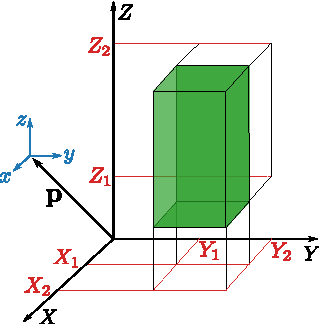
\includegraphics[width=0.6\linewidth]{figs/rectangular-prism.pdf}
    \caption{
        Prisma rectangular y punto de observación $\mathbf{p}$ definidos en un
        sistema de coordenadas Cartesianas $\{X, Y, Z\}$. Se define un sistema
        de coordenadas Cartesianas $\{x, y, z\}$ con origen en el punto de
        observación $\mathbf{p}$ y con ejes paralelos a $X, Y, Z$,
        respectivamente.
    }
    \label{fig:rectangular-prism}
\end{figure}

Con el objetivo de simplificar los cálculos, definimos un sistema de
coordenadas Cartesianas $\{x, y, z\}$ cuyo origen se encuentra en el punto de
observación $\mathbf{p}$ y sus ejes son paralelos a los del sistema $\{X, Y,
Z\}$, respectivamente (Fig.~\ref{fig:rectangular-prism}).
Los vértices del prisma vendrán dados por las coordenadas
$x_1, x_2, y_1, y_2, z_1, z_2$ en el nuevo sistema de referencia, es decir:

\begin{equation}
    \begin{aligned}
        x_1 &= X_1 - X, & x_2 &= X_2 - X, \\
        y_1 &= Y_1 - Y, & y_2 &= Y_2 - Y, \\
        z_1 &= Z_1 - Z, & z_2 &= Z_2 - Z.
    \end{aligned}
\end{equation}

Bajo este nuevo sistema de referencia, el potencial gravitatorio se puede
expresar como:

\begin{equation}
    V(\mathbf{p}) =
    G \rho
    \int\limits_{x_1}^{x_2}
    \int\limits_{y_1}^{y_2}
    \int\limits_{z_1}^{z_2}
    \frac{\diff x' \diff y' \diff z'}{\sqrt{{x'}^2 + {y'}^2 + {z'}^2}}.
\end{equation}

El resultado de esta integración posee la siguiente forma
\citep{nagy2000,nagy2002}:

\begin{equation}
    \begin{split}
        V(\mathbf{p}) =
        G \rho
        \Bigg[ &
            xy \ln (z + l) + yz \ln(x + l) + zx \ln(y + l) \\
               &
            - \frac{x^2}{2} \arctan \frac{yz}{xl}
            - \frac{y^2}{2} \arctan \frac{zx}{yl}
            - \frac{z^2}{2} \arctan \frac{xy}{zl}
        \Bigg]
        \Bigg|_{x_1}^{x_2}
        \Bigg|_{y_1}^{y_2}
        \Bigg|_{z_1}^{z_2},
    \end{split}
    \label{eq:potencial-prismas-analitico}
\end{equation}

\noindent donde

\begin{equation}
    l = \sqrt{x^2 + y^2 + z^2}.
\end{equation}

Reemplazando todos los límites del dominio de integración, obtenemos un total
de 48 términos.
A la hora de evaluarlos numéricamente hay que tener en cuenta que la solución
analítica de la ecuación~\ref{eq:potencial-prismas-analitico} no es
continua en todo $\mathbb{R}^3$, particularmente en los casos en los que el
punto de observación se encuentra sobre alguno de los vértices, aristas o caras
del prisma ($x_{1,2}=0$, $y_{1,2}=0$ ó $z_{1,2}=0$). Sin embargo el potencial
$V(\mathbf{p})$ sí lo es.
Para solucionar esto, es necesario reemplazar aquellos términos que no pueden
ser evaluados por sus límites cuando $(x, y, z) \rightarrow (0, 0, 0)$
\citep{nagy2000}.
Por ejemplo:

\begin{equation}
    \lim_{(x, y, z)\rightarrow (0, 0, 0)} xz \ln(z + r) = 0.
\end{equation}

Una solución alternativa es reemplazar la función $\ln$ por una nueva función
$\safelog(x)$ definida de la siguiente manera:

\begin{equation}
    \safelog(x) =
    \begin{cases}
        \ln(x) & \quad x \ge x_\text{umbral} \\
        0      & \quad x < x_\text{umbral}
    \end{cases}
    \label{eq:safe_log}
\end{equation}

\noindent donde $x_\text{umbral}$ es un valor muy pequeño del argumento de
$\safelog$ a partir del cual consideramos que la función debe ser evaluada en
su límite en cero.
La elección de este valor dependerá de las dimensiones del problema que estamos
resolviendo.
En el caso de un modelado directo geofísico, en el cual las dimensiones de los
primas vienen dadas por varios metros, podemos asumir un valor de
$x_\text{umbral} = 10^{-10}$m \citep{harmonica2021}.

Por otro lado, la evaluación de la función $\arctan$ requiere ciertos cuidados.
Para que el potencial $V(\mathbf{p})$ satisfaga la ecuación de Poisson
(ec.~\ref{eq:potencial-poisson}), es necesario utilizar la siguiente forma de
la función $\safearctan(y, x)$ \citep{fukushima2020}:

\begin{equation}
    \safearctan(y, x) =
    \begin{cases}
        \arctan(y / x) & \quad x \ne 0 \\
        \pi / 2        & \quad x = 0,\, y > 0 \\
        -\pi / 2       & \quad x = 0,\, y < 0 \\
        0              & \quad x = 0,\, y = 0.
    \end{cases}
    \label{eq:safe_arctan}
\end{equation}

Haciendo uso de las funciones $\safelog$ y $\safearctan$ definidas en las
ecuaciones~\ref{eq:safe_log} y \ref{eq:safe_arctan}, respectivamente, el
potencial gravitatorio generado por un prisma rectangular en cualquier punto de
observación $\mathbf{p}$ puede ser numéricamente calculado mediante:

\begin{equation}
    \begin{split}
        V(\mathbf{p}) =
        G \rho
        \Bigg[ &
            xy \safelog (z + l)
            + yz \safelog(x + l)
            + zx \safelog(y + l)
           - \frac{x^2}{2} \safearctan(yz, xl)
                \\&
           - \frac{y^2}{2} \safearctan(zx, yl)
           - \frac{z^2}{2} \safearctan(xy, zl)
        \Bigg]
        \Bigg|_{x_1}^{x_2}
        \Bigg|_{y_1}^{y_2}
        \Bigg|_{z_1}^{z_2}.
    \end{split}
    \label{eq:potencial-prismas-numerico}
\end{equation}

De manera análoga, podemos calcular las componentes del gradiente del potencial
gravitatorio generado por un prisma rectangular haciendo uso de las siguientes
expresiones \citep{nagy2000,nagy2002}:

\begin{align}
    g_x(\mathbf{p}) =&
        \Big[
            y \safelog(z + l) + z \safelog(y + l)  - x \safearctan(yz, xl)
        \Big]
        \Big|_{x_1}^{x_2}
        \Big|_{y_1}^{y_2}
        \Big|_{z_1}^{z_2} \\
    g_y(\mathbf{p}) =&
        \Big[
            z \safelog(x + l) + x \safelog(z + l)  - y \safearctan(zx, yl)
        \Big]
        \Big|_{x_1}^{x_2}
        \Big|_{y_1}^{y_2}
        \Big|_{z_1}^{z_2} \\
    g_z(\mathbf{p}) =&
        \Big[
            x \safelog(y + l) + y \safelog(x + l) - z \safearctan(xy, zl)
        \Big]
        \Big|_{x_1}^{x_2}
        \Big|_{y_1}^{y_2}
        \Big|_{z_1}^{z_2}.
\end{align}


\subsection{Tesseroides}

En caso de querer realizar modelos directos de estructuras regionales,
continentales o globales, el uso de prismas rectangulares en coordenadas
Cartesianas no resulta la mejor opción, ya que no tienen en cuenta la curvatura
del planeta Tierra.
La mayoría de los modelos directos que sí lo hacen se definen en coordenadas
esféricas geocéntricas y consisten en discretizar la Tierra en geometrías
simples.
Este es el caso de los \emph{tesseroides} \citep{anderson1976}, también
conocidos como prismas esféricos, los cuales se definen como el volumen
comprendido entre dos esferas de radios distintos, dos meridianos de longitudes
distintas y dos paralelos de distintas latitudes (Fig.~\ref{fig:tesseroid}).

\begin{figure}
    \centering
    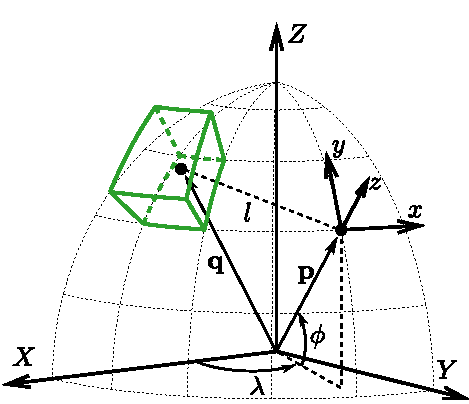
\includegraphics[width=0.7\linewidth]{figs/tesseroid-coord-sys.pdf}
    \caption{
        Tesseroide (prisma esférico) en un sistema de coordenadas esféricas
        geocéntricas, junto a un punto de cómputo situado en $\mathbf{p}$ y su
        correspondiente sistema \emph{local} de coordenadas Cartesianas.
        Obtenida de \citet{uieda2015}.
    }
    \label{fig:tesseroid}
\end{figure}

El potencial gravitatorio que genera un tesseroide de densidad uniforme $\rho$,
definido por las coordenadas $r_1$, $r_2$, $\lambda_1$, $\lambda_2$, $\phi_1$
y $\phi_2$, sobre un punto de observación $\mathbf{p}$, dado por las
coordenadas esféricas $r$, $\lambda$ y $\phi$, se puede obtener aplicando estos
límites de integración a la ecuación~\ref{eq:potencial-gravitatorio-integral},
quedando expresado como la siguiente integral volumétrica
\citep{grombein2013,uieda2016}:

\begin{equation}
    V(\mathbf{p}) = G \rho
        \int\limits_{r_1}^{r_2}
        \int\limits_{\lambda_1}^{\lambda_2}
        \int\limits_{\phi_1}^{\phi_2}
        \frac{\kappa}{\left\lVert \mathbf{p} - \mathbf{q} \right\rVert}
        \diff r' \diff \lambda' \diff \phi',
    \label{eq:potencial-tesseroide}
\end{equation}

\noindent donde

\begin{equation}
    \kappa = {r'}^2 \cos \phi',
    \label{eq:kappa}
\end{equation}

\noindent la distancia $\left\lVert \mathbf{p} - \mathbf{q} \right\rVert$ viene
dada por la ecuación~\ref{eq:distance-spherical} y las coordenadas de
integración $r'$, $\lambda'$ y $\phi'$ representan la posición $\mathbf{q}$ de
cada volumen infinitesimal del tesseroide.

Reemplazando los límites de integración de las ecuaciones \ref{eq:gx-integral},
\ref{eq:gy-integral} y \ref{eq:gz-integral} por los del tesseroide, podemos
obtener las componentes del gradiente del potencial gravitatorio generado por
el tesseroide en el punto de observación $\mathbf{p}$ con respecto al
sistema de coordenadas \emph{local}:

\begin{align}
    g_x(\mathbf{p}) &=
        G \rho
        \int\limits_{r_1}^{r_2}
        \int\limits_{\lambda_1}^{\lambda_2}
        \int\limits_{\phi_1}^{\phi_2}
        \frac{\Delta x}{\left\lVert \mathbf{p} - \mathbf{q} \right\rVert^3}
        \kappa
        \diff r' \diff \lambda' \diff \phi',
    \label{eq:gx-tesseroide}
    \\
    g_y(\mathbf{p}) &=
        G \rho
        \int\limits_{r_1}^{r_2}
        \int\limits_{\lambda_1}^{\lambda_2}
        \int\limits_{\phi_1}^{\phi_2}
        \frac{\Delta y}{\left\lVert \mathbf{p} - \mathbf{q} \right\rVert^3}
        \kappa
        \diff r' \diff \lambda' \diff \phi',
    \label{eq:gy-tesseroide}
    \\
    g_z(\mathbf{p}) &=
        G \rho
        \int\limits_{r_1}^{r_2}
        \int\limits_{\lambda_1}^{\lambda_2}
        \int\limits_{\phi_1}^{\phi_2}
        \frac{\Delta z}{\left\lVert \mathbf{p} - \mathbf{q} \right\rVert^3}
        \kappa
        \diff r' \diff \lambda' \diff \phi',
    \label{eq:gz-tesseroide}
\end{align}

\noindent donde $\Delta x$, $\Delta y$ y $\Delta z$ vienen dadas por las
ecuaciones~\ref{eq:delta-x}, \ref{eq:delta-y} y \ref{eq:delta-z},
respectivamente.

Las ecuaciones~\ref{eq:potencial-tesseroide}, \ref{eq:gx-tesseroide},
\ref{eq:gy-tesseroide} y \ref{eq:gz-tesseroide} contienen integrales elípticas
que no poseen solución analítica y deben ser aproximadas numéricamente.
Existen dos principales métodos en la literatura para aproximar estas
integrales: uno involucra expansiones en serie de Taylor
\citep{heck2006,grombein2013} mientras que los otros hacen uso de la \ac{GLQ}
\citep{asgharzadeh2007,wildpfeiffer2008,li2011,uieda2016,lin2018}.
En el Capítulo~\ref{cha:tesseroids-variable-density} se detallan las razones
por las cuales a lo largo de esta Tesis abordaremos la estrategia de la
\ac{GLQ}.

La \Ac{GLQ} consiste en la aproximación de una integral por una suma ponderada
del integrando evaluado en determinadas abscisas
\citep[][p.~390]{hildebrand1987}:

\begin{equation}
    \int\limits_{-1}^1 f(x) \diff x \approx
        \sum\limits_{i=1}^{N} W_i f(x_i),
\end{equation}

\noindent donde $N$ es el órden de la cuadratura,
$x_i$ corresponden a las raíces del polinomio de Legendre $P_N(x)$ de grado
$N$, y $W_i$ son los pesos ponderados de cada término:

\begin{equation}
    W_i = \frac{2}{(1 - x_i^2) \Big[ P'_N(x_i) \Big]^2}.
\end{equation}

\noindent El polinomio de Legendre $P_N(x)$ se puede obtener mediante
relaciones de recurrencia \citep[][p.~330]{hildebrand1987}:

\begin{align}
    &P_0(x) = 1 \\
    &P_1(x) = x \\
    &P_{N + 1}(x) = \frac{2N + 1}{N + 1} x P_N(x) - \frac{N}{N + 1}P_{N-1}(x).
\end{align}

\noindent
Mientras que los valores que asume su primera derivada $P'_N(x)$ en las raíces
$x_i$ se pueden obtener gracias a la siguiente relación
\citep[][p.~391]{hildebrand1987}:

\begin{equation}
    P'_N(x_i) = \frac{N}{(1 - x_i^2)} P_{N - 1}(x_i).
\end{equation}

La Tabla~\ref{tab:legendre-roots} muestra las raíces de los primeros polinomios
de Legendre y sus respectivos pesos ponderados.

\begin{table}
    \centering
    \caption{
        Raíces de algunos polinomios de Legendre junto con los correspondientes
        pesos ponderados a ser utilizados en la \ac{GLQ}
        \citep[][p.~392]{hildebrand1987}.
    }
    \begin{tabular}{ccc}
        \hline
        Orden ($N$) & Raíces ($x_i$)                                     & Pesos ponderados ($W_i$)    \\
        \hline
        1     & 0                                                        & 2                           \\
        2     & $\pm \frac{1}{\sqrt{3}}$                                 & 1                           \\
        3     & 0                                                        & $\frac{8}{9}$               \\
              & $\pm \sqrt{\frac{3}{5}}$                                 & $\frac{5}{9}$               \\
        4     & $\pm \sqrt{\frac{3}{7} - \frac{2}{7}\sqrt{\frac{6}{5}}}$ & $\frac{18 + \sqrt{30}}{36}$ \\
              & $\pm \sqrt{\frac{3}{7} + \frac{2}{7}\sqrt{\frac{6}{5}}}$ & $\frac{18 - \sqrt{30}}{36}$
    \end{tabular}
    \label{tab:legendre-roots}
\end{table}

En el caso de que la integral posea límites de integración distintos a
$(-1, 1)$, podemos escalar los nodos y aplicar la \ac{GLQ} de la siguiente
forma:

\begin{equation}
    \int\limits_a^b f(x) \diff x \approx
        \frac{b - a}{2} \sum\limits_{i=1}^{N}
        W_i f(x_i^s),
\end{equation}

\noindent donde

\begin{equation}
    x_i^s = \frac{b - a}{2} x_i + \frac{b + a}{2}.
\end{equation}

Haciendo uso de la \ac{GLQ}, podemos aproximar las integrales volumétricas de
las ecuaciones~\ref{eq:potencial-tesseroide}, \ref{eq:gx-tesseroide},
\ref{eq:gy-tesseroide}, \ref{eq:gz-tesseroide} de la siguiente manera
\citep{asgharzadeh2007,uieda2016}:

\begin{equation}
    \int\limits_{r_1}^{r_2}
    \int\limits_{\lambda_1}^{\lambda_2}
    \int\limits_{\phi_1}^{\phi_2}
    f(r', \lambda', \phi')
    \diff r' \diff \lambda' \diff \phi' =
    A
    \sum\limits_{i=1}^{N_r}
    \sum\limits_{j=1}^{N_\lambda}
    \sum\limits_{k=1}^{N_\phi}
    W_i^r
    W_j^\lambda
    W_k^\phi
    f(r_i, \lambda_j, \phi_j),
    \label{eq:glq-integral-volumetrica}
\end{equation}

\noindent donde

\begin{equation}
    A = \frac{
        (r_2 - r_1) (\lambda_2 - \lambda_1) (\phi_2 - \phi_1)
    }{8},
    \label{eq:glq-resize-factor}
\end{equation}

\noindent $N_r$, $N_\lambda$ y $N_\phi$ son los órdenes de la cuadratura en
cada dirección; $r_i$, $\lambda_j$ y $\phi_k$ representan los nodos escalados
de las cuadraturas para cada dirección; y $W_i^r$, $W_j^\lambda$, $W_k^\phi$
sus respectivos pesos ponderados.

Como se puede observar en la ecuación~\ref{eq:glq-integral-volumetrica}, la
\ac{GLQ} aproxima el campo gravitatorio de un tesseroide por el que genera
un conjunto de masas puntuales situadas en los nodos escalados de los
polinomios de Legendre.
La precisión de la aproximación dependerá entonces de la cantidad de nodos
utilizados en las sumatorias, es decir, de los órdenes de las cuadraturas.
Es posible entonces aumentar la precisión de la \ac{GLQ} incrementando los
órdenes de las cuadraturas.
Sin embargo, el aumento de los órdenes de la cuadratura incrementa la cantidad
de nodos según $O(n^3)$, haciendo de esta estrategia un método muy ineficiente.

\citet{ku1977} demostró que la precisión de la aproximación también depende del
cociente entre la distancia al punto de observación y la distancia entre nodos
adyacentes.
Haciendo uso de esto, \citet{li2011} han propuesto un método más eficiente para
aumentar la precisión de la aproximación manteniendo: la \emph{discretización
adaptativa}.
Esta consiste en mantener el orden de las cuadraturas constantes e ir
dividiendo el tesseroide en otros tesseroides de menor tamaño según la
distancia entre ellos y el punto de observación.
De esta forma, se incrementa la cantidad de nodos en las regiones que mayor
afectan a la precisión, obteniendo un número considerablemente menor de nodos
pero manteniendo una buena precisión.
En el Capítulo \ref{cha:tesseroids-variable-density} describiremos en detalle
la \emph{discretización adaptativa}.


% =============================================================================

\section{Gravedad terrestre}
\label{sec:gravedad-terrestre}

Un cuerpo en reposo situado sobre la superficie de la Tierra experimenta una
fuerza resultante de la suma de la fuerza de atracción gravitatoria (debida
a la masa del planeta) y la fuerza centrífuga, debida a la rotación del planeta
sobre su eje y al sistema de referencia no inercial donde se encuentra dicho
cuerpo.
Esta fuerza genera sobre el cuerpo una aceleración $\mathbf{g}$ que
llamaremos \emph{gravedad}, a partir de la cual podemos definir un
\emph{campo de gravedad} $W$:

\begin{equation}
    \nabla W(\mathbf{p}) = +\mathbf{g}(\mathbf{p}).
    \label{eq:campo-gravedad-terrestre}
\end{equation}

El \emph{campo de gravedad} $W$ puede ser expresado como:

\begin{equation}
    W(\mathbf{p}) = V(\mathbf{p}) + \Phi(\mathbf{p}),
\end{equation}

\noindent donde $V(\mathbf{p})$ es el \emph{potencial gravitatorio} que genera
la Tierra sobre el punto $\mathbf{p}$
(ecuación~\ref{eq:potencial-gravitatorio-integral}), y $\Phi(\mathbf{p})$ el
\emph{potencial centrífugo} al cual se ve sometido el cuerpo situado en el
punto $\mathbf{p}$ debido a la rotación del planeta.
Este último puede expresarse como:

\begin{equation}
    \Phi(\mathbf{p}) = \frac{1}{2} \omega^2 (X^2 + Y^2),
    \label{eq:potencial-centrifugo}
\end{equation}

\noindent donde $\omega$ es el módulo de la velocidad angular de rotación de la
Tierra y $X$ e $Y$ son las coordenadas horizontales del punto $\mathbf{p}$ en
un sistema de referencia Cartesiano geocéntrico
(Fig.~\ref{fig:spherical-coordinates}).

Vale notar que el potencial $W$ no es un campo harmónico, ya que no satisface
la ecuación de Poisson (ec.~\ref{eq:potencial-poisson}). En cambio, se rige
acorde a una \emph{ecuación de Poisson generalizada}:

\begin{equation}
    \nabla^2 W(\mathbf{p}) = - 4\pi G \rho(\mathbf{p}) + 2 \omega^2.
\end{equation}

Las superficies

\begin{equation}
    W(\mathbf{p}) = \text{const},
\end{equation}

\noindent se definen como \emph{superficies equipotenciales}.

A partir de la definición del vector de \emph{gravedad}
(ec.~\ref{eq:campo-gravedad-terrestre}), es posible deducir que
$\mathbf{g}(\mathbf{p})$ es un vector normal a la superficie equipotencial que
pasa por el mismo punto $\mathbf{p}$.
Cada una de las curvas que cortan normalmente a las superficies equipotenciales
se definen como \emph{líneas de fuerza} o \emph{líneas de campo}
(\emph{plumb lines} en inglés).

La superficie equipotencial que coincide con el nivel medio del mar se define
como el \emph{geoide}:

\begin{equation}
    W(\mathbf{p}) = W_0.
\end{equation}

\noindent El geoide nos permite definir la \emph{altitud ortométrica} $H$ de
cualquier punto $\mathbf{p}$ como la distancia entre la superficie del geoide
y el punto $\mathbf{p}$ medida a lo largo de la línea de fuerza que pasa por el
mismo punto $\mathbf{p}$ (Fig.~\ref{fig:superficies-equipotenciales}).


\subsection{Gravedad normal}

Las mediciones del campo gravitatorio terrestre nos permite obtener información
acerca de las masas que componen nuestro planeta. Los valores de este campo
presentan ligeras variaciones a lo largo de la Tierra, originadas por la
diferentes densidades de las masas del interior del planeta. Debido a que estas
variaciones suelen ser lo suficientemente pequeñas, es posible asociarlas a la
presencia de \emph{cuerpos anómalos} bajo la superficie terrestre. Para poder
identificarlos es necesario definir primero el concepto de \emph{Tierra
normal}.

En una primera aproximación podemos considerar la geometría de la Tierra como
un elipsoide de revolución. Si bien esta aproximación no es lo suficientemente
apropiada para muchas aplicaciones, nos provee de una descripción matemática
sencilla, cuyas derivaciones poseen soluciones analíticas.
De esta manera definiremos a la \emph{Tierra normal} como un \emph{elipsoide de
referencia}, es decir, un elipsoide de revolución que representa una superficie
equipotencial del campo de gravedad que este genera. Llamaremos $U(\mathbf{p})$
al \emph{campo de gravedad normal}, es decir, el potencial de gravedad generado
por el elipsoide de referencia y definimos al elipsoide de referencia como la
siguiente superficie equipotencial:

\begin{equation}
    U(\mathbf{p}) = U_0 = \text{cte}.
\end{equation}

El campo de gravedad normal puede ser escrito como

\begin{equation}
    U(\mathbf{p}) = V_\text{el}(\mathbf{p}) + \Phi(\mathbf{p}),
\end{equation}

\noindent donde $\Phi(\mathbf{p})$ es el potencial centrífugo debido a la
rotación del elipsoide de revolución (ec.~\ref{eq:potencial-centrifugo})
y $V_\text{el}(\mathbf{p})$ es el potencial gravitatorio que produce el mismo
elipsoide.

El elipsoide de referencia vendrá definido mediante los siguientes parámetros:

\begin{enumerate}
    \item{la forma del elipsoide, dada por los dos semiejes $a$ y $b$,}
    \item{la masa total $M$ del elipsoide, y}
    \item{la velocidad angular $\omega$.}
\end{enumerate}

\noindent A partir de ellos podemos describir la superficie del elipsoide como:

\begin{equation}
    \frac{X^2 + Y^2}{a^2} + \frac{Z^2}{b^2} = 1
\end{equation}

\noindent donde $X$, $Y$ y $Z$ son coordenadas Cartesianas geocéntricas.

Vale notar que no resulta indispensable definir la distribución de densidad del
elipsoide \citep[][p.~64]{heiskanen1967}.

El elipsoide de referencia no solo nos permite tener un modelo de \emph{Tierra
normal}, sino que además nos permite definir un nuevo sistema de coordenadas:
las \emph{coordenadas geodésicas} o \emph{geográficas}.
Dado un punto arbitrario $\mathbf{p}$ podemos especificar su ubicación mediante
su \emph{longitud} $\lambda$, su
\emph{latitud geodésica}\footnote{%
    Se notará a la \emph{latitud geodésica} con $\varphi$ y a la \emph{latitud
    esférica} con $\phi$.
}
$\varphi$ y su \emph{altitud geométrica} $h$.
El ángulo longitudinal $\lambda$ coincide con la longitud del punto
$\mathbf{p}$ desde un sistema de coordenadas esféricas.
La altura geométrica $h$ corresponde a la distancia entre el punto $\mathbf{p}$
y la superficie del elipsoide a lo largo de línea de fuerza del potencial $U$
que pasa por el punto $\mathbf{p}$ (Fig.~\ref{fig:coordenadas-geodesicas}).
Debido a las propiedades del potencial $U$ sus líneas de fuerza todas
rectas que cortan normalmente a cada una de sus superficies equipotenciales.
Por ende, la altitud geométrica $h$ equivale a la longitud del segmento de
recta que une el punto $\mathbf{p}$ con la superficie del elipsoide a lo largo
de la dirección normal al mismo.
La latitud geodésica corresponde al ángulo comprendido entre el plano
ecuatorial y la prolongación de una recta normal al la superficie del elipsoide
que pasa por el punto $\mathbf{p}$ (Fig.~\ref{fig:coordenadas-geodesicas}).

\begin{figure}
    \centering
    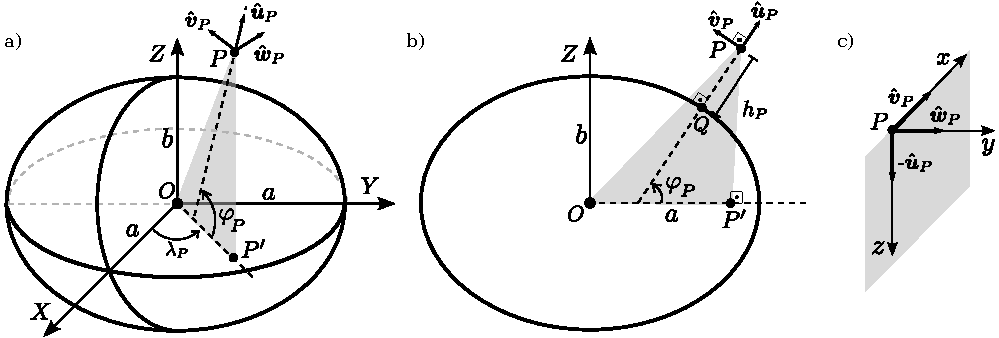
\includegraphics[width=\linewidth]{figs/cartesian-geodetic-systems.pdf}
    \caption{
        Elipsoide de referencia y coordenadas geodésicas del punto
        $\mathbf{p}$.
        (a)~Elipsoide de referencia definido por los
        semiejes $a$ y $b$, junto con un sistema
        Cartesiano geocéntrico $\{X, Y, Z\}$. Se observan los ángulos
        longitudinal $\lambda$ y latitudinal $\varphi$ del punto
        $\mathbf{p}$.
        (b)~Sección del elipsoide por el plano que contiene al punto
        $\mathbf{p}$. Se destaca el punto $\mathbf{q}$ correspondiente
        a la intersección de la superficie del elipsoide con la línea de
        fuerza que pasa por el punto $\mathbf{p}$.
        Se observan la latitud geodésica $\varphi$, la latitud esférica
        $\phi$ y la altitud geométrica $h$ del punto $\mathbf{p}$.
        Esta figura es una versión modificada de \citet{oliveira2021}.
    }
    \label{fig:coordenadas-geodesicas}
\end{figure}

Definiremos el \emph{vector gravedad normal} $\boldsymbol\gamma$ como el
gradiente del campo de gravedad normal:

\begin{equation}
    \boldsymbol\gamma(\mathbf{p}) = \nabla U(\mathbf{p}).
\end{equation}

Vale notar que el gradiente de un campo en un punto $\mathbf{p}$ consiste en un
vector normal a la superficie equipotencial a la cual pertenece el punto
$\mathbf{p}$.
De esta manera, al calcular el gradiente del campo de gravedad normal desde el
sistema de coordenadas geodésicas podemos deducir que sólo la componente
normal es no nula \citep[][p.~68]{heiskanen1967}, es decir:

\begin{equation}
    \gamma_\lambda =
        \frac{\partial U}{\partial \lambda} = 0  \quad
    \gamma_\varphi =
        \frac{\partial U}{\partial \varphi} = 0.
\end{equation}

Definimos la \emph{gravedad normal} como el módulo del vector de gravedad
normal:

\begin{equation}
    \gamma(\mathbf{p}) = | \gamma_h(\mathbf{p}) | =
        \frac{\partial U(\mathbf{p})}{\partial h}.
\end{equation}

Dada la simetría de rotación del elipsoide y el hecho que el potencial
centrífugo no depende de la posición longitudinal, la gravedad normal depende
únicamente de la altitud geométrica y la latitud geodésica del punto
$\mathbf{p}$.

\subsubsection{Fórmula cerrada}
\label{sec:normal-gravity-closed-form}

Existe una expresión analítica para la gravedad normal en cualquier punto
externo al elipsoide de referencia dada por la \emph{fórmula cerrada} (del
inglés \emph{closed-form formula}) de \citet{li2001a}:


\begin{equation}
    \gamma(\varphi, h) =
    \frac{1}{\Omega}
    \Bigg\{
        \frac{G M}{{b'}^2 + E^2}
        + \frac{\omega^2 a^2 E q'}{({b'}^2 + E^2) q_0}
        \Bigg(
            \frac{1}{2}
            \sin^2 \beta' - \frac{1}{6}
        \Bigg)
        - \omega^2 b' \cos^2 \beta'
    \Bigg\},
    \label{eq:normal-gravity-closed-form}
\end{equation}

\noindent donde

\begin{align}
    E &= \sqrt{a^2 - b^2}
        \quad \text{es la \emph{excentricidad lineal}}, \\
    \Omega &= \sqrt{\frac{{b'}^2 + E^2 \sin^2 \beta'}{{b'}^2 + E^2}}, \\
    q' &= 3
        \left(1 + \frac{{b'}^2}{E^2} \right)
        \left(1 - \frac{b'}{E} \arctan \frac{E}{b'} \right)
        - 1, \\
    q_0 &= \frac{1}{2}
        \left[
            \left(
                1 + \frac{3b^2}{E^2}
            \right)
            \arctan \frac{E}{b} - \frac{3b}{E}
        \right], \\
    b' &= \sqrt{{r''}^2 - E^2 \cos^2 \beta'}, \\
    \cos \beta' &= \sqrt{
        \frac{1}{2}
        + \frac{R}{2}
        - \sqrt{
            \frac{1}{4} + \frac{R^2}{4}  - \frac{D}{2}
        }
    },
\end{align}

\noindent y

\begin{align}
    R &= \frac{{r''}^2}{E^2}, \\
    D &= \frac{{d''}^2}{E^2}, \\
    {r''}^2 &= {r'}^2 + {z'}^2, \\
    {d''}^2 &= {r'}^2 - {z'}^2, \\
    r' &= a\cos\beta + h\cos\varphi, \\
    z' &= b\sin\beta + h\sin\varphi, \\
    \tan\beta &= \frac{b}{a}\tan\varphi.
\end{align}

La \emph{fórmula cerrada} para la gravedad normal de la
ecuación~\ref{eq:normal-gravity-closed-form} nos permite calcular
analíticamente la gravedad normal generada por el elipsoide de revolución sobre
cualquier punto exterior al mismo.

\subsubsection{Ecuación de Somigliana}

Como caso particular, la gravedad normal en cualquier punto situado sobre la
superficie del elipsoide de referencia ($h=0$) se puede calcular de manera
sencilla a través de la ecuación de Somigliana \citep{heiskanen1967}:

\begin{equation}
    \gamma(\varphi, h=0) =
        \gamma_e
        \frac{1 + k \sin^2\varphi}{\sqrt{1 - e^2 \sin^2\varphi}};
    \label{eq:somigliana}
\end{equation}

\noindent donde

\begin{equation}
    k = \frac{b}{a} \frac{\gamma_p}{\gamma_e} - 1;
\end{equation}

\noindent $e$ es la \emph{primera excentricidad}

\begin{equation}
    e = \sqrt{\frac{a^2 - b^2}{a^2}};
\end{equation}

\noindent y $\gamma_e$ y $\gamma_p$ son los valores de la gravedad normal en
cualquier punto del ecuador y en los polos, respectivamente
(ver~\citealp[][p.~68--69,]{heiskanen1967} para más detalles).


\subsection{Disturbio de gravedad}

Con el objeto de poder identificar y caracterizar la distribución de densidades
anómalas en el interior de la Tierra, es necesario remover la \emph{gravedad
normal} de la gravedad terrestre.
Definiremos entonces al \emph{vector del disturbio de gravedad}
$\boldsymbol\delta \mathbf{g}$ (\emph{gravity disturbance vector} en inglés)
como la diferencia entre el vector \emph{gravedad} en el punto $\mathbf{p}$
y el vector \emph{gravedad normal} calculado en el mismo punto $\mathbf{p}$
(Fig.~\ref{fig:superficies-equipotenciales}):

\begin{equation}
    \boldsymbol\delta \mathbf{g}(\mathbf{p}) =
        \mathbf{g}(\mathbf{p}) - \boldsymbol\gamma(\mathbf{p}).
    \label{eq:gravity-disturbance-vector}
\end{equation}

\begin{figure}[t!]
    \centering
    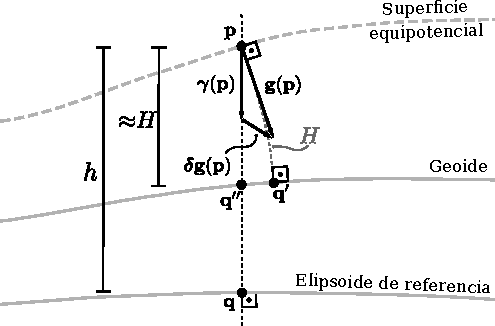
\includegraphics[width=\linewidth]{figs/surfaces.pdf}
    \caption{
        Elipsoide de referencia, geoide y vector del disturbio de gravedad.
        Se identifica un punto $\mathbf{p}$ situado a una altitud geométrica
        $h$ indicada por el segmento de recta que une el punto $\mathbf{q}$
        sobre el elipsoide de referencia.
        Se observa el vector de gravedad $\mathbf{g}(\mathbf{p})$ sobre el
        punto $\mathbf{p}$ normal a la superficie equipotencial del campo de
        gravedad $W$ que pasa por el mismo punto $\mathbf{p}$.
        Se identifica además el vector de gravedad normal
        $\boldsymbol\gamma(\mathbf{p})$ y el vector de disturbio de gravedad
        $\boldsymbol\delta \mathbf{g}(\mathbf{p})$.
        La altitud ortométrica $H$ se determina por la longitud del segmento de
        la línea de fuerza del potencial $W$ que une el punto $\mathbf{q'}$
        sobre el geoide con el punto $\mathbf{p}$, aunque puede aproximarse por
        el segmento de recta que une el punto $\mathbf{q''}$ y el punto
        $\mathbf{p}$.
        Las curvaturas de las superficies equipotenciales han sido exageradas
        para mejorar la visualización.
        Esta figura es una versión modificada de \citet{oliveira2021b}.
    }
    \label{fig:superficies-equipotenciales}
\end{figure}

La mayoría de las metodologías que nos permiten realizar mediciones del campo
gravitatorio terrestre consiguen estimar el valor de la componente del vector
$\mathbf{g}$ a lo largo de la línea de fuerza del campo de gravedad $W$, la
cual coincide con el módulo de $\mathbf{g}$.
Medir la dirección del vector $\mathbf{g}$ resulta un problema de mayor
complejidad, dificultando el cálculo del \emph{vector del disturbio de
gravedad}.
Es por ello que introducimos el concepto del \emph{disturbio de gravedad}
$\delta g$ (\emph{gravity disturbance} en inglés), definido como la diferencia
entre el módulo del vector gravedad y el módulo del vector gravedad normal en
el mismo punto $\mathbf{p}$
\citep{heiskanen1967,hofmannwellenhof2005,oliveira2018}:

\begin{equation}
    \delta g(\mathbf{p}) =
        g(\mathbf{p}) - \gamma(\mathbf{p}).
    \label{eq:gravity-disturbance}
\end{equation}

Vale notar que el \emph{disturbio de gravedad} $\delta g$ no coincide con el
módulo del \emph{vector disturbio de gravedad} $\boldsymbol\delta \mathbf{g}$
\citep{barthelmes2013,sanso2013,oliveira2018}.
Sin embargo, se puede asumir que el \emph{disturbio de gravedad} se aproxima lo
suficiente al módulo del \emph{vector del disturbio de gravedad} si
consideramos que la desviación del vector $\mathbf{g}(\mathbf{p})$ de la recta
normal al elipsoide en el punto $\mathbf{p}$ es lo suficientemente pequeña.

% =============================================================================

\section{Fuentes equivalentes}

Consideremos una distribución de masa arbitraria limitada a una región $\Omega$
con una densidad $\rho$ y un punto de observación $\mathbf{p}$ exterior a la
región $\Omega$ (Fig.~\ref{fig:fuentes-equivalentes}).
El potencial gravitatorio $V$ que genera la distribución de masa en el punto
$\mathbf{p}$ puede calcularse a través de la ecuación
\ref{eq:potencial-gravitatorio-integral}.

Consideremos además una superficie equipotencial arbitraria $\partial S$ de
forma tal que el punto $\mathbf{p}$ se encuentra fuera de la región $S$
interior a $\partial S$ (Fig.~\ref{fig:fuentes-equivalentes}).
Vamos a asumir que el potencial $V$ toma un valor constante $V_S$ en
$\partial S$.
Aplicando la segunda identidad de Green \citep[][p.~23]{blakely1995} podemos
obtener:

\begin{equation}
    \begin{split}
    \int\limits_S
        \Bigg[
            V(\mathbf{q}) \,
            \nabla^2 \left( \frac{1}{\left\lVert \mathbf{p} - \mathbf{q}
                \right\rVert} \right)
            - \frac{1}{\left\lVert \mathbf{p} - \mathbf{q} \right\rVert}
            \nabla^2 V(\mathbf{q})
        \Bigg]
    \diff v
    = \\
    \oint\limits_{\partial S}
        \Bigg[
            V(\mathbf{q}) \,
            \frac{\partial}{\partial n}
            \left(
                \frac{1}{\left\lVert \mathbf{p} - \mathbf{q} \right\rVert}
            \right)
            -
            \frac{1}{\left\lVert \mathbf{p} - \mathbf{q} \right\rVert}
            &\frac{\partial V}{\partial n}
        \Bigg]
    \diff s,
    \end{split}
\end{equation}

\noindent donde $\mathbf{q}$ es la variable de integración en ambos miembros
y $n$ indica la dirección normal a la superficie $\partial S$.

El primer término de la integral volumétrica es nulo, ya que la inversa de
$\left\lVert \mathbf{p} - \mathbf{q} \right\rVert$ es un campo harmónico.
Por otro lado, el valor de $V(\mathbf{q})$ en el primer término de la integral
de superficie es constante, ya que el dominio de integración $\partial S$ es
una superficie equipotencial de $V$.
Por lo tanto, la ecuación anterior puede expresarse de forma más sencilla como:

\begin{equation}
    - \int\limits_S
        \frac{\nabla^2 V(\mathbf{q})}{\left\lVert \mathbf{p} - \mathbf{q}
            \right\rVert}
    \diff v
    =
    V_S
    \oint\limits_{\partial S}
        \frac{\partial}{\partial n}
        \left(
            \frac{1}{\left\lVert \mathbf{p} - \mathbf{q} \right\rVert}
        \right)
    \diff s
    - \oint\limits_{\partial S}
        \frac{1}{\left\lVert \mathbf{p} - \mathbf{q} \right\rVert}
        \frac{\partial V}{\partial n}
    \diff s.
\end{equation}

Uno de los corolarios de la primera identidad de Green establece que la
integral de la derivada normal de una función harmónica  sobre una superficie
cerrada es nula \citep[][p.~20]{blakely1995}. Por ende podemos anular la
primera integral de superficie de la ecuación anterior:

\begin{equation}
    - \int\limits_S
        \frac{\nabla^2 V(\mathbf{q})}{\left\lVert \mathbf{p} - \mathbf{q}
            \right\rVert}
    \diff v
    =
    - \oint\limits_{\partial S}
        \frac{1}{\left\lVert \mathbf{p} - \mathbf{q} \right\rVert}
        \frac{\partial V}{\partial n}
    \diff s,
\end{equation}

Si aplicamos la ecuación de Poisson (ec.~\ref{eq:potencial-poisson})
y definimos una densidad superficial $\sigma$:

\begin{equation}
    \sigma(\mathbf{q}) =
    \frac{-1}{4\pi G} \frac{\partial V}{\partial n},
\end{equation}

\noindent podemos expresar la ecuación anterior como:

\begin{equation}
    G \int\limits_S
        \frac{\rho(\mathbf{q})}{\left\lVert \mathbf{p} - \mathbf{q}
            \right\rVert}
    \diff v
    =
    G \oint\limits_{\partial S}
        \frac{\sigma(\mathbf{q})}{\left\lVert \mathbf{p} - \mathbf{q}
            \right\rVert}
    \diff s.
\end{equation}

\begin{figure}[t]
    \centering
    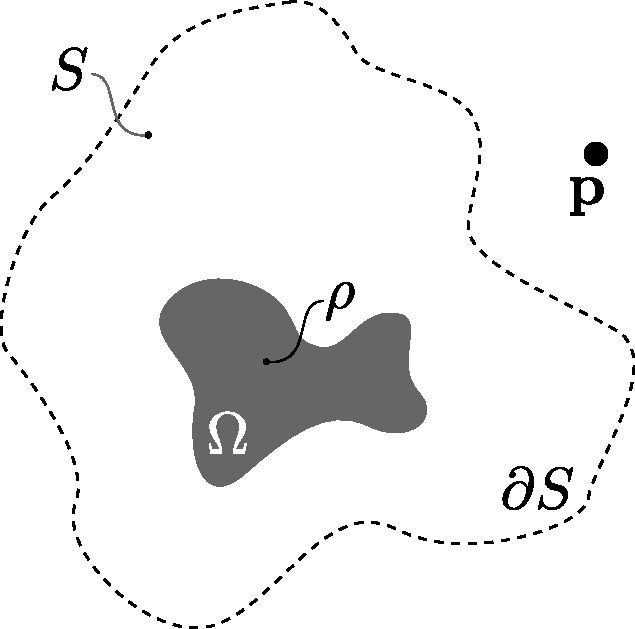
\includegraphics[width=0.4\linewidth]{figs/fuentes-equivalentes.pdf}
    \caption{
        Distribución de masa tridimensional con densidad $\rho$ dentro de una
        región $\Omega$, junto con superficie equipotencial $\partial S$ del
        campo gravitatorio generado por la misma y un punto de observación
        $\mathbf{p}$ exterior a la región $S$ interior a $\partial S$.
    }
    \label{fig:fuentes-equivalentes}
\end{figure}

Considerando que la densidad $\rho$ es nula fuera de la región $\Omega$,
podemos simplificar el dominio de integración de la integral volumétrica.
De esta manera, ambos términos equivalen al valor que asume el potencial $V$ en
el punto $\mathbf{p}$ (ec.~\ref{eq:potencial-gravitatorio-integral}):

\begin{equation}
    V(\mathbf{p}) =
    G \int\limits_\Omega
        \frac{\rho(\mathbf{q})}{\left\lVert \mathbf{p} - \mathbf{q}
            \right\rVert}
    \diff v
    =
    G \oint\limits_{\partial S}
        \frac{\sigma(\mathbf{q})}{\left\lVert \mathbf{p} - \mathbf{q}
            \right\rVert}
    \diff s.
\end{equation}

Esta relación se conoce como \emph{fuentes equivalentes de Green}
(\emph{Green's equivalent layer} en inglés) y de la cual se deduce que el
potencial que genera una distribución de densidad tridimensional es
indistinguible del que genera una masa superficial (o una capa delgada)
distribuida sobre una superficie equipotencial \citep[][p.~62]{blakely1995}.

Esta propiedad de los campos gravitatorios nos permite desarrollar metodologías
de interpolación de campos harmónicos basados en el modelado de distribuciones
de masas arbitrarias, sin necesidad de que guarden relación con las geometrías
y densidades de los cuerpos que generan los campos observados.
Además, las fuentes equivalentes de Green dejan en evidencia la no unicidad de
las fuentes de los campos gravitatorios: existe una infinita cantidad de
distribuciones de masas que pueden generar el mismo campo gravitatorio, o una
aproximación suficiente para resultar indistinguible a efectos prácticos.
